% IISA 2026 - 8 page Full Paper
% 17th International Conference on Information, Intelligence, Systems and Applications
% IEEE Conference Format
%
\documentclass[conference]{IEEEtran}

\usepackage[T1]{fontenc}
\usepackage[utf8]{inputenc}
\usepackage{graphicx}
\usepackage{hyperref}
\usepackage[dvipsnames]{xcolor}
\usepackage{booktabs}
\usepackage{multirow}
\usepackage{amsmath}
\usepackage{amssymb}
\usepackage{url}
\usepackage{cite}
\usepackage{balance}
\usepackage{tikz}
\usepackage{subcaption}
\usepackage{amsmath} % For math symbols
\usetikzlibrary{positioning, arrows.meta, shapes.geometric, calc, backgrounds, fit}

\usepackage{caption}
\captionsetup{font=footnotesize}

\usepackage{tipa}  % Provides phonetic symbols including eng (Ŋ/ŋ)

\usepackage{etoolbox}
\setlength{\textfloatsep}{8pt plus 2pt minus 2pt}
\setlength{\intextsep}{8pt plus 2pt minus 2pt}  % for [h]/[H] placement
\setlength{\floatsep}{8pt plus 2pt minus 2pt}

% For special Sami characters
\usepackage{newunicodechar}
\DeclareUnicodeCharacter{014A}{\raisebox{0.1ex}{\scalebox{1.3}{\textipa{\ng}}}}  % Ŋ (capital eng - scaled)
\DeclareUnicodeCharacter{014B}{\textipa{\ng}}  % ŋ (lowercase eng)
% \DeclareUnicodeCharacter{0166}{\={T}}  % Ŧ (approximation using macron)
% \DeclareUnicodeCharacter{0167}{\={t}}  % ŧ
% T-stroke: horizontal bar through the letter (not macron above)
\newcommand{\tstroke}{\mbox{\ooalign{t\cr\hspace{0.02em}\raisebox{0.49ex}{\rule{0.30em}{0.4pt}}}}}
\newcommand{\Tstroke}{\mbox{\ooalign{T\cr\hspace{0.04em}\raisebox{0.52ex}{\rule{0.52em}{0.45pt}}}}}
\DeclareUnicodeCharacter{0166}{\Tstroke}  % Ŧ (T with stroke through)
\DeclareUnicodeCharacter{0167}{\tstroke}  % ŧ (t with stroke through)
\DeclareUnicodeCharacter{0110}{\DJ}  % Đ (uses T1's \DJ)
\DeclareUnicodeCharacter{0111}{\dj}  % đ (uses T1's \dj)

% ============================================================================
% BENCHMARK RESULTS MACROS - From benchmark_results.json
% ============================================================================
% Best TrOCR model (trocr_smi_synth)
\newcommand{\trocrBestCER}{8.55}
% \newcommand{\trocrBestWER}{27.51}
\newcommand{\trocrBestWER}{28.16}
\newcommand{\trocrBestCharAcc}{91.45}  % 100 - CER (8.55)
\newcommand{\trocrBestWordAcc}{71.84}  % 100 - WER (28.16)
\newcommand{\trocrBestTime}{12.41}
\newcommand{\trocrSize}{350}

% Our CNN-CTC model (ctc_simple)
\newcommand{\preprocessingImgWidth}{800}
\newcommand{\ctcCER}{12.24}
% \newcommand{\ctcWER}{37.55}
\newcommand{\ctcWER}{37.35}
\newcommand{\ctcCharAcc}{87.76}  % 100 - CER (12.24)
\newcommand{\ctcWordAcc}{62.65}  % 100 - WER (37.35)
\newcommand{\ctcTime}{0.033}
\newcommand{\ctcSize}{23}

% Speed comparison
\newcommand{\speedupFactor}{380}

% Other TrOCR variants (benchmark results - main table)
\newcommand{\trocrSmiPredSynthCER}{15.85}
\newcommand{\trocrSmiPredSynthWER}{45.76}
\newcommand{\trocrSmiPredSynthWordAcc}{54.24}  % 100 - WER (45.76)
\newcommand{\trocrSmiPredSynthTime}{12.08}
\newcommand{\trocrSmiNorPredSynthCER}{17.46}
\newcommand{\trocrSmiNorPredSynthWER}{48.20}
\newcommand{\trocrSmiNorPredSynthWordAcc}{51.80}  % 100 - WER (48.20)
\newcommand{\trocrSmiNorPredSynthTime}{13.55}
\newcommand{\trocrSmiCER}{24.12}
\newcommand{\trocrSmiWER}{63.50}
\newcommand{\trocrSmiWordAcc}{36.50}  % 100 - WER (63.50)
\newcommand{\trocrSmiTime}{16.23}

% Dataset statistics
\newcommand{\trainSamples}{276,000}
\newcommand{\testSamples}{1,048}
\newcommand{\hfTestSamples}{1,000}
\newcommand{\hfValidationSamples}{31,000}
\newcommand{\bookTestSamples}{48}
\newcommand{\charsetSize}{395}

% Book data results
\newcommand{\ctcBookCER}{12.21}
\newcommand{\trocrBookCER}{17.35}

% Domain specific performance (Table: HF vs Book)
\newcommand{\trocrSynthHFCER}{8.33}
\newcommand{\trocrSynthBookCER}{13.17}
\newcommand{\trocrSynthDeltaCER}{4.84}
\newcommand{\trocrSynthBookNormAcc}{45.8}
\newcommand{\ctcBookNormAcc}{62.5}
\newcommand{\trocrPredSynthHFCER}{16.09}
\newcommand{\trocrPredSynthBookCER}{11.00}
\newcommand{\trocrPredSynthDeltaCER}{5.09}
\newcommand{\trocrPredSynthBookNormAcc}{43.8}

% Split experiment results
\newcommand{\splitLongOriginalCER}{15.17}
\newcommand{\splitLongSplitCER}{8.12}
\newcommand{\splitShortCER}{12.04}
\newcommand{\splitImprovement}{7.05}
\newcommand{\splitPValue}{0.000009}
\newcommand{\splitCohensD}{1.35}
\newcommand{\splitSamplesSplit}{20}
\newcommand{\splitLongCount}{67}
\newcommand{\splitImproveRate}{95}

% End to end pipeline
\newcommand{\bleuScore}{10.40}
\newcommand{\chrfScore}{33.85}
\newcommand{\terScore}{76.30}

\newcommand{\inferencetime}{10 to 15}

% Derived metrics and constants
\newcommand{\cerGap}{3.69}
\newcommand{\sizeRatio}{15}
\newcommand{\ctcThroughputK}{109}  % thousands of images per hour (3600/0.033 ≈ 109K)
\newcommand{\trocrThroughput}{290}  % images per hour (3600/12.41 ≈ 290)
\newcommand{\millionPagesCtcHours}{10}  % 1M / 109K ≈ 9.2 hours, rounded up
\newcommand{\millionPagesTrocrDays}{144}  % 1M / (290 * 24) ≈ 144 days
\newcommand{\sentenceLengthThreshold}{80}
\newcommand{\imageHeight}{32}
\newcommand{\hiddenDim}{256}
\newcommand{\lstmOutputDim}{512}
\newcommand{\numParams}{6}
\newcommand{\turiYear}{1910}
\newcommand{\smiSpeakers}{25,000}
\newcommand{\numCharsVocab}{394}
\newcommand{\trocrInferenceIntroSec}{12}

\begin{document}

% ============================================================================
% TITLE
% ============================================================================
% \title{Digitization of Endangered Low-Resource S\'{a}mi Languages: OCR-Translation Pipeline}
\title{Lightweight OCR in North S\'{a}mi Heritage Digitization for Smart Learning}
% Language as Living Hertiage: Digitialization Methods for Endangered Low-Resource Sami Languages
% 

% ============================================================================
% AUTHORS
% ============================================================================
\author{
\IEEEauthorblockN{Jan Musio\l{}\IEEEauthorrefmark{1}, Aparna S. Varde\IEEEauthorrefmark{2}, and Juan Heredia\IEEEauthorrefmark{3}}
\IEEEauthorblockA{University of Southern Denmark\\
\IEEEauthorrefmark{1}S\o nderborg, \IEEEauthorrefmark{2}Vejle, \IEEEauthorrefmark{3}Odense, Denmark\\
Email: jamus23@student.sdu.dk, \{apva, jehm\}@mmmi.sdu.dk}
}
%
% \institute{University of Southern Denmark (1. Sondenborg, 2. Vejle, 3. Odense), Denmark\\

\maketitle

% ============================================================================
% ABSTRACT (~150 to 200 words)
% ============================================================================
\begin{abstract}
North S\'{a}mi is an endangered Uralic language, facing critical challenges in written heritage preservation. State-of-the-art Transformer-based OCR (Optical Character Recognition) models get \trocrBestCharAcc{}\% accuracy, but need \trocrSize{} MB+ storage and over \trocrInferenceIntroSec{} seconds for inference on a single image on a CPU, which limits their practicality, especially in resource-constrained digitization. In this research, we propose a model comprising a lightweight integrated pipeline of a CNN-CTC (Convolutional Neural Network and  Connectionist Temporal Classification) architecture to conduct OCR of S\'{a}mi language texts with resource-aware transcription.  We offer systematic evaluation of our proposed CNN-CTC model (comparing it to 7 TrOCR variants from National Library of Norway), testing on \testSamples{} North S\'{a}mi text samples, including synthetically rendered historical content in Johan Turi's \turiYear{} work. Our CNN-CTC model gives \ctcCharAcc\% character accuracy, trailing the best Transformer by \cerGap{}\,pp in CER, while operating \speedupFactor{} times faster, taking only \ctcSize{} MB, enabling throughput of \ctcThroughputK{},000 images per hour compared to \trocrThroughput{} for Transformers. We observe that the CNN-CTC model maintains stable accuracy when tested on synthetically rendered historical text where a transformer model degrades by \trocrSynthDeltaCER{}\,pp. %while our model remains stable.
Additionally, we demonstrate that linguistically motivated conjunction-based sentence splitting improves long sentence accuracy by \splitImprovement{}\,pp as a proof of concept for preprocessing-based mitigation. Through our findings we infer that an efficient deployable OCR for low-resource language digitization is achievable without sacrificing practical accuracy, supporting community-driven preservation efforts. 
%The performance on physical scan degradation remains untested as all evaluation used synthetic renderings. 

\end{abstract}

\begin{IEEEkeywords}
AI in Education, CNN-CTC, Culture for Smart Cities, Heritage Digitization, Indigenous \& Low-Resource Languages, 
NLP, OCR, Smart Learning \& Living, Sustainable AI 
\end{IEEEkeywords}

% ============================================================================
% I. INTRODUCTION (~0.8 pages)
% ============================================================================
\section{Introduction}
\label{sec:introduction}

The S\'{a}mi languages comprise nine low-resource languages that belong to the family of Uralic languages. They are spoken in the S\'{a}pmi region, spread over the countries of Norway, Sweden, Finland, and Russia. 
North S\'{a}mi (Davvis\'{a}megiella) is the most widely spoken, with approximately \smiSpeakers{} speakers, yet it remains classified as endangered by UNESCO.
Throughout history, the governments of these countries have systematically suppressed the native population~\cite{minde2003}. Norway has adopted the most aggressive strategy (Fornorsking\footnote{eng. Norwegianization}), banning the language, confiscating land and material goods, sending settlers to the S\'{a}pmi region and dislocating the indigenous communities. Other countries employed different discrimination techniques such as forced assimilation and relocation of indigenous people, collectivization and assertion of their material goods. 
Nowadays, the Nordic countries, by and large, have acknowledged their mistakes and are actively participating in the revitalization of the S\'{a}mi languages\footnote{Norway's parliament issued a formal apology in November 2024, after the June 2023 Truth and Reconciliation report.}. 

The preservation of S\'{a}mi languages now depends critically on digitizing historical documents before they deteriorate.
Optical Character Recognition (OCR) is essential for this effort, yet most mainstream OCR research focuses on high-resource languages, leaving S\'{a}mi underrepresented, putting historical texts at risk.
Effective OCR not only preserves heritage but also enables modern language technology applications essential for language revitalization. 

North S\'{a}mi presents significant challenges for OCR systems.
The scarcity of digital resources, special diacritical characters (\'{A}/\'{a}, \v{C}/\v{c}, Đ/đ, Ŋ/ŋ, \v{S}/\v{s}, Ŧ/ŧ, \v{Z}/\v{z}), its agglutinative morphology, large vocabulary with hundreds of inflected forms per verb and a cross-linguistically rare three-way quantity contrast complicate the character recognition for S\'{a}mi orthography. Figure~\ref{fig:sami_example} illustrates these challenges with an example sentence from Johan Turi's 1910 work and seven special diacritical characters.

% \vspace{-0.5cm}
% \begin{figure}[h]
% \centering
% % \vspace{-0.3cm}
% 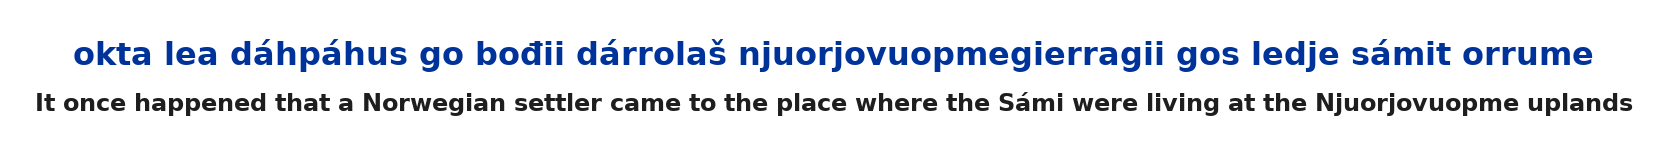
\includegraphics[width=0.50\textwidth]{figures/entry_80.png}
% % \footnotesize
% % \vspace{-0.3cm}
% \caption{Example sentence from Johan Turi's ``Muitalus s\'{a}miid birra''~\cite{turi1910} with translation.}
% % "\textit{It once happened that a Norwegian settler came to the place where the Sámi were living at the Njuorjovuopme uplands.}"
% \label{fig:example}
% \end{figure}
% % \vspace{-0.7cm}
% % \normalsize
% \begin{figure}[h]
% \centering
% 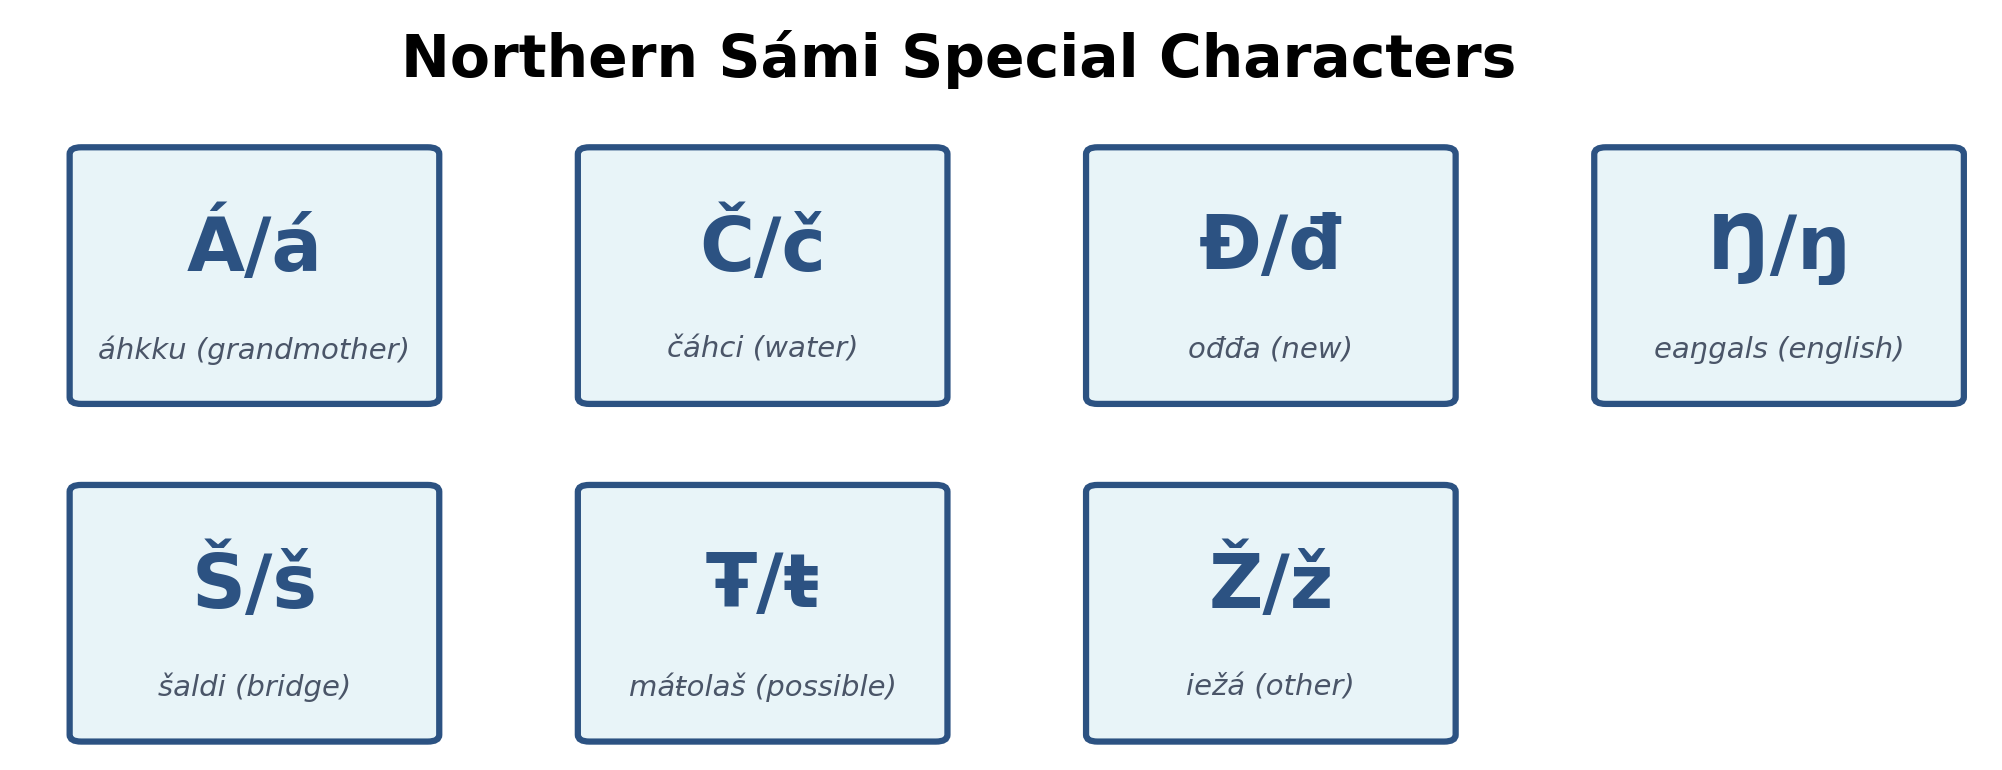
\includegraphics[width=0.85\columnwidth]{figures/sami_alphabet_cut.png}
% \caption{North S\'{a}mi special characters with example words. These seven diacritical characters distinguish S\'{a}mi orthography from standard Latin and pose recognition challenges for OCR systems.}
% \label{fig:alphabet}
% \end{figure}

\begin{figure}[h]
\centering
% 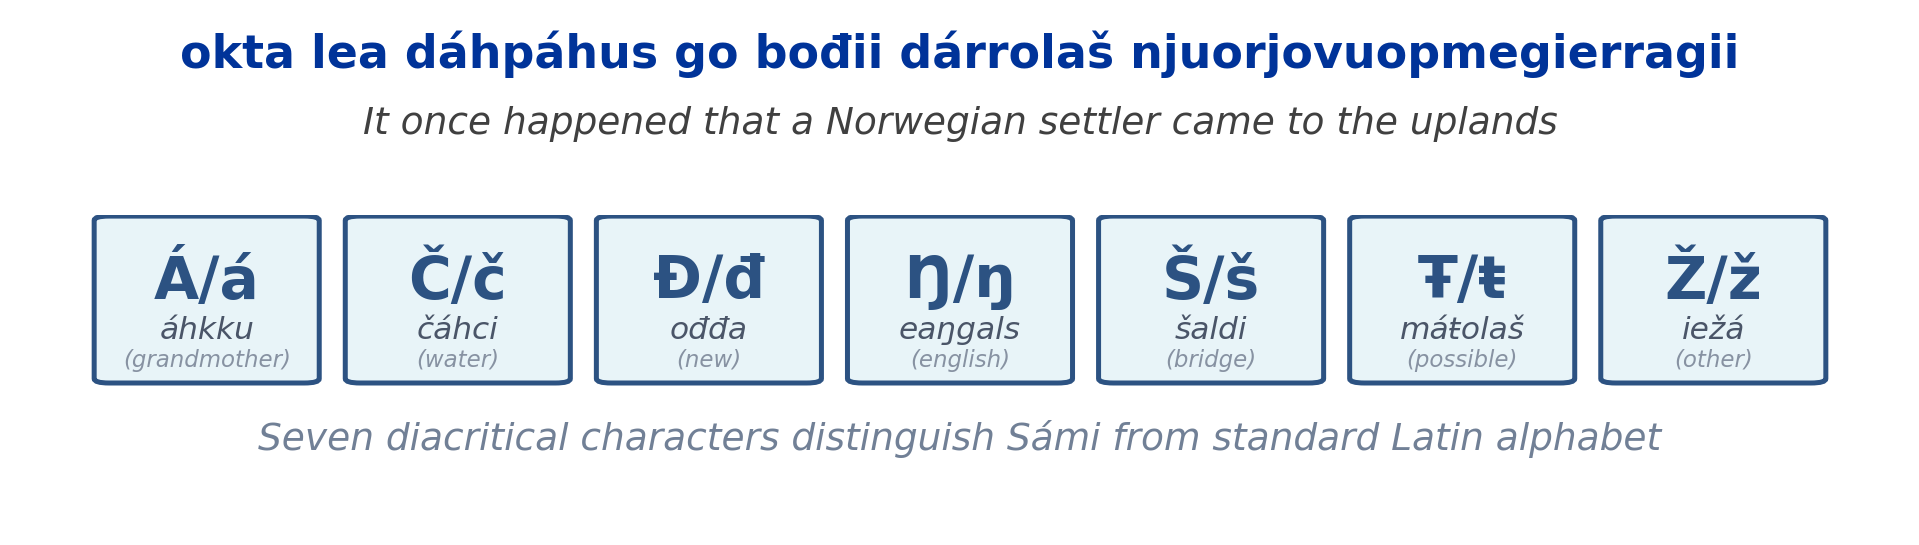
\includegraphics[width=\columnwidth]{figures/combined_example.png}
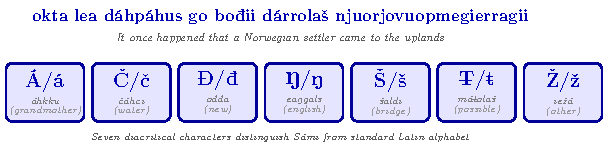
\includegraphics[width=\columnwidth]{figures/combined_intro.pdf}
\caption{\footnotesize North S\'{a}mi text characteristics: (a) Example sentence from Johan Turi's ``Muitalus s\'{a}miid birra''~\cite{turi1910} with English translation, and (b) Seven special diacritical characters with example words that distinguish S\'{a}mi orthography from standard Latin script.}
\label{fig:sami_example}
\end{figure}

Current state-of-the-art (SOTA) models from the National Library of Norway utilize transformer-based architecture ~\cite{li2023trocr} leveraging pre-training on large-scale datasets, fine-tuned for S\'{a}mi languages~\cite{enstad2025}. These are computationally demanding and time-consuming (\trocrSize{}MB+ model size with CPU inference times exceeding \trocrInferenceIntroSec{} seconds per image). This limits their applicability in resource-constrained environments such as community-driven projects or institutions with limited infrastructure. Moreover, Enstad et al.~\cite{enstad2025} found that current baseline OCR accuracy remains insufficient for downstream NLP tasks, highlighting the need for both improved accuracy and practical deployment solutions. 

In this paper, we propose a lightweight CNN-CTC model for resource-aware transcription of S\'{a}mi language text. It thus contributes to sustainable AI. It impacts AI for 21st-century education, especially with respect to culture for smart cities and ethnic plurality, by working on low-resource indigenous language texts. This research aids smart learning and smart living. It can be useful in augmenting AI systems with NLP (natural language processing) for low-resource languages, and in training next-generation robots for everyday use (e.g. grocery stores, household use) by operating on indigenous language texts. 
% We answer the question whether a more lightweight solution exists. We compare the results against the state-of-the-art models. 
This paper thus addresses a vital question: \textit{Can a lightweight OCR architecture approach Transformer level accuracy for North S\'{a}mi while enabling practical deployment on modest hardware?} The main contributions of this work are:

\begin{enumerate}
    \item Proposing a CNN-CTC model for resource-aware OCR transcription of North S\'{a}mi language texts with implementation on notable benchmark data \& historical texts. %from Johan Turi's \turiYear{} work ``Muitalus s\'{a}miid birra''~\cite{turi1910}. 
    \item Approaching SOTA accuracy within \cerGap{}\,pp CER across 7 TrOCR variants on \testSamples{} samples, while surpassing them in speed, size, and out-of-domain accuracy.
    \item Impacting Sustainable AI through a lightweight CNN-CTC model (\ctcSize{} MB) with \ctcCharAcc\% character accuracy, \speedupFactor{}$\times$ faster inference than most Transformers.
    \item Adding a linguistically motivated conjunction splitting approach that improves long sentence accuracy by \splitImprovement{}\,pp as a proof of concept.
    \item Aiding Smart Learning by an end-to-end pipeline integrating OCR \& machine translation (BLEU \bleuScore{}, chrF \chrfScore{}, TER \terScore{}\%), good for document processing.  
    \item Usefulness in 21st-century education, AI \& NLP, and next-gen robotic systems on low-resource languages. 
\end{enumerate}
% ============================================================================
% II. RELATED WORK (~1.2 pages)
% ============================================================================
\section{Related Work}
\label{sec:related_work}

\subsection{OCR for Low-Resource Languages}
OCR research has traditionally focused on high-resource languages with abundant training data. Recently, more focus has been put onto low-resource setting. Agarwal and Anastasopoulos~\cite{agarwal2024ocr} provide a concise survey of OCR methods for low-resource languages, highlighting transfer learning, synthetic data generation and architecture adaptation. Rijhwani et al.~\cite{rijhwani2020} demonstrated OCR post-correction for endangered languages using pretrained language models, while Corallo and Varde~\cite{corallo2023} addressed OCR for Amazigh (Berber), another low-resource language with distinctive orthography. The OCR4MT benchmark~\cite{ignat2022ocr4mt} ties OCR for 60 low-resource languages directly to downstream MT performance.
For morphologically rich languages, the vocabulary explosion problem affects both OCR confidence and language model integration. Approaches include subword tokenization~\cite{sennrich2016bpe} and character-level modeling, the latter being relevant for CTC-based architectures that operate at the character level by design.

\subsection{Neural OCR Architectures}
\label{subsec:neural_ocr}
There are two Neural Network based approaches for OCR.
First, a classical approach exemplified by CRNN~\cite{shi2017crnn}, which combines a Convolutional Neural Network (CNN) for feature extraction and Recurrent Neural Network (RNN) for sequence modeling, trained with Connectionist Temporal Classification (CTC) loss. CTC allows alignment of length-varying sequences, therefore eliminating the need for explicit segmentation. The CRNN is efficient, explainable, and end-to-end trainable.  
The second approach employs Transformer architecture~\cite{vaswani2017attention} either as encoders (e.g. Vision Transformer~\cite{dosovitskiy2020vit}) or encoder-decoder models. 
TrOCR~\cite{li2023trocr} by Microsoft represents the state of the art using a Vision Transformer encoder pre-trained on large image datasets and a language model decoder. National Library of Norway has fine-tuned TrOCR variants for S\'{a}mi languages~\cite{enstad2025}. While achieving better accuracy, TrOCR models are computationally expensive and time-consuming (often exceeding \inferencetime  sec/image on CPU and taking \trocrSize{} MB).

\subsection{S\'{a}mi Language Technology}
\label{subsec:sami_tech}
%Several initiatives support S\'{a}mi language technology development.

The TartuNLP research group at University of Tartu provides a neural machine translation API~\cite{tartunlp} supporting North S\'{a}mi to English translation (used in this work's end-to-end pipeline). The National Library of Norway, via the Spr\r{a}kbanken initiative, released synthetic OCR training data and fine-tuned TrOCR models for S\'{a}mi~\cite{enstad2025}. The Giellatekno project at UiT The Arctic University of Norway maintains morphological analyzers, lexical entries for many languages, proofing tools and language-learning system~\cite{moshagen2014} and contributed synthetic OCR training data, through the Spr\r{a}kbanken initiative.
Despite these advances, deployment challenges remain: Transformer models computational demands limit accessibility for resource-constrained digitization projects. Our work addresses this gap on whether lightweight architectures can provide practical accuracy-efficiency trade-offs for heritage document processing.
% ============================================================================
% III. NORTH SAMI LANGUAGE AND DATA (~0.8 pages)
% ============================================================================
\section{North S\'{a}mi Language and Data}
\label{sec:data}

\subsection{Linguistic Characteristics}
\label{subsec:linguistic}
The S\'{a}mi language family consists of 9 languages (Southern, Ume, Pite, Lule, Northern, Inari, Skolt, Kildin, Ter)~\cite{sammallahti1998}. It is an Uralic language family of the Finno-Ugric branch, sharing typological features with Finnish and Hungarian. 
Its orthography, standardized in 1970s, uses the Latin alphabet augmented with seven special characters: \'{a}, \v{c}, đ, ŋ, \v{s}, ŧ, and \v{z} (and their corresponding capitals). These characters present challenges for OCR systems: the háček (\v{}) may be confused with similar diacritics, while đ and ŧ have no visual analogs in major European languages. Additionally, North S\'{a}mi's agglutinative morphology produces large type-token ratios even in modest corpora, complicating n-gram language models used in OCR post-correction and creating vocabulary challenges for character recognition systems.

\subsection{Training Data}
\label{subsec:training_data}

For training, we use the Spr\r{a}kbanken synthetic S\'{a}mi OCR dataset~\cite{enstad2025}, available through the Hugging Face Hub. We load the dataset's \textit{training split} (307,387 samples) and divide it into a \textit{training subset} (\trainSamples{} images, 90\%) for model optimization and a \textit{development subset} (approximately \hfValidationSamples{} images, 10\%) for hyperparameter tuning and early stopping. 
Each image is 32$\times$800 pixels (height$\times$width) with corresponding ground truth transcription, generated from digital text using varied fonts, sizes, and mild distortions to simulate scanned documents. Synthetic data is necessary because no publicly available, large-scale corpus of real scanned North S\'{a}mi documents with ground truth exists. Additionally, it opens a door for recreating the approach for other low-resource languages. The character vocabulary comprises \numCharsVocab{} unique characters covering uppercase and lowercase Latin letters, S\'{a}mi-specific characters, digits, punctuation, and common symbols, plus one CTC blank token, for \charsetSize{} output classes in total. This vocabulary size reflects the linguistic diversity of the corpus while remaining feasible for CTC-based decoding.

\subsection{Test Data}
\label{subsec:test_data}

Evaluation employs test sets to assess in-domain \& out-of-domain generalization, distinct from training sets and unused for hyperparameter tuning / early stopping.

\textbf{Spr\r{a}kbanken Test Subset:} \hfTestSamples{} synthetic line images randomly sampled from the dataset creators' separate \textit{validation split}. This set measures in-domain accuracy on data matching the training distribution but never seen by the model, distinct from the development subset mentioned above.

\textbf{Historical Book Data:} \bookTestSamples{} hand-picked, synthetically rendered sentence pairs in Johan Turi's ``Muitalus s\'{a}miid birra'' (An Account of the S\'{a}mi, 1910)~\cite{turi1910}, the first secular book published in North S\'{a}mi. Images were generated using varied fonts and rendering parameters to evaluate out-of-domain generalization. It tests lexical and morphological generalization to historical vocabulary, not scan quality robustness.

The complete test set comprises \testSamples{} samples: \hfTestSamples{} from the Spr\r{a}kbanken held-out split plus \bookTestSamples{} historical book samples. 


% ============================================================================
% IV. METHODOLOGY (~2.0 pages)
% ============================================================================
\section{Methodology}
\label{sec:methodology}

\subsection{System Overview}
\label{subsec:system_overview}


 Our modular OCR pipeline is structured as follows: the images are preprocessed, they pass through a CNN backbone for feature extraction, followed by adaptive pooling and projection to a fixed hidden dimension. These features are then passed directly to a linear classification head and decoded via CTC loss~\cite{graves2006ctc}. Figure~\ref{fig:architecture} illustrates this architecture.
 The modular design supports different backbone (SimpleCNN, VGG16, VGG19, ResNet50, with ResNet101 in the design space but gated on the ResNet50 result and not trained due to compute) and encoder (BiLSTM, Transformer, None) combinations, enabling systematic comparison of the architectures. Due to time constraints, this work only evaluates the no encoder CTC variant type (CNN $\rightarrow$ projection $\rightarrow$ CTC head).
\begin{figure}[tb]

    \centering
    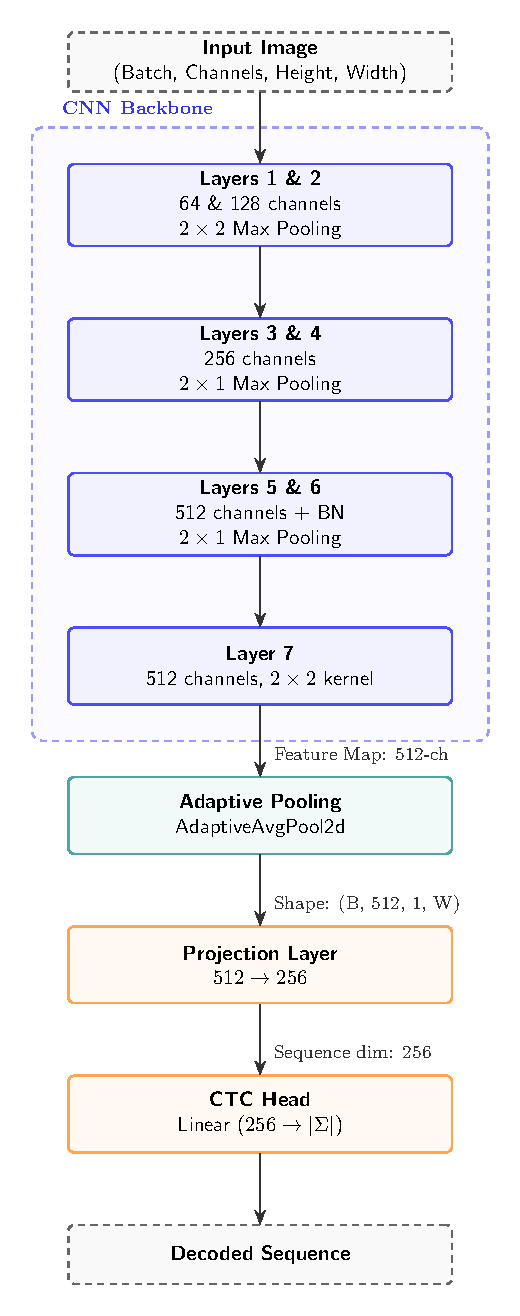
\includegraphics[width=\columnwidth, height=0.7\textheight, keepaspectratio]{figures/architecture_tikz.pdf}
        \footnotesize 
    \caption{Modular OCR pipeline CNN-CTC architecture. Input images (\imageHeight{}$\times$\preprocessingImgWidth{} pixels) are processed through a CNN backbone, pooled to height 1, and projected to hidden dimension \hiddenDim{}, the projected column features are passed directly to the CTC head to produce character sequences.}
    \label{fig:architecture}
\end{figure}


\subsection{Image Preprocessing}
\label{subsec:preprocessing}

Input images undergo grayscale conversion, aspect-ratio-preserving resize to \imageHeight{} pixels height, and width normalization (padding or cropping) to \preprocessingImgWidth{} pixels. Pixel values are normalized from [0, 255] to [-1, 1] via $(x/255 - 0.5) / 0.5$. During training, random affine transformations (rotation $\pm$2\textdegree, translation/scale $\pm$2\%) and ColorJitter (brightness=0.2, contrast=0.2) simulate scanning variations.

\subsection{CNN-CTC Architecture}
\label{subsec:cnn_ctc}

In line with the needs of resource-aware systems, our lightweight model (\textit{ctc\_simple}) proposes to deploy a simple CNN backbone trained from scratch:

\textbf{7 layer CNN backbone}:
\begin{itemize}
    \item Layers 1,2: 64,128 channels, 2$\times$2 max pooling
    \item Layers 3,4: 256 channels, 2$\times$1 pooling (preserved width)
    \item Layers 5,6: 512 channels, batch normalized, 2$\times$1 pooling
    \item Layer 7: 512 channels, 2$\times$2 kernel (height reduced to 1)

    % \item \textbf{Layers 0 to 1:} Conv3x3(64) + ReLU + MaxPool(2,2), Conv3x3(128) + ReLU + MaxPool(2,2)
    % \item \textbf{Layers 2 to 3:} Conv3x3(256) + ReLU, Conv3x3(256) + ReLU + MaxPool(2,1)
    % \item \textbf{Layers 4 to 5:} Conv3x3(512) + BatchNorm + ReLU, Conv3x3(512) + BatchNorm + ReLU + MaxPool(2,1)
    % \item \textbf{Layer 6:} Conv2x2(512) + ReLU (no padding)
\end{itemize}

This CNN backbone is preferred due to prior success stories, e.g. it renders good results in work by Shi et al.~\cite{shi2017crnn}. 

\textbf{Subsampling:} MaxPool operations use stride (2,2) for early layers and (2,1) for later layers to preserve horizontal resolution while collapsing height. The output is a 512 channel feature map of reduced spatial dimensions.

\textbf{Adaptive Pooling:} Features are pooled to height 1 via AdaptiveAvgPool2d, yielding a tensor of shape (batch, 512, 1, \textit{width}). \textit{Width} depends on input width and pooling reductions.

\textbf{Projection Layer:} A linear transformation projects the \lstmOutputDim{} dimensional CNN features (512 backbone channels) to a hidden size of \hiddenDim{}.

\textbf{Sequence Stage:} For \textit{ctc\_simple}, no recurrent or attention based encoder is applied, the projected column features are passed directly to the CTC head. This isolates the contribution of the backbone alone and yields the lightest variant of the modular pipeline.

\textbf{CTC Decoder:} A linear layer projects the \hiddenDim{} dimensional column features to \charsetSize{} classes (\numCharsVocab{} characters + 1 CTC blank token), followed by LogSoftmax. During training, CTC loss marginalizes over all valid character-level alignments, at inference, greedy decoding or beam search extracts the most likely character sequence.

% remove the repeated section?
% \textbf{Model Size:} The complete architecture contains approximately \numParams{} million parameters, resulting in a \ctcSize{}MB checkpoint file—\sizeRatio{}$\times$ smaller than TrOCR's \trocrSize{}MB.

\subsection{Comparison Architectures}
\label{subsec:comparison}

We evaluate 11 models (7 TrOCR + 4 CTC) variants across different backbones and encoders:

Seven TrOCR variants, pretrained by the National Library of Norway~\cite{enstad2025}, use a Vision Transformer encoder and GPT-2 decoder: \textit{trocr\_smi} (base S\'{a}mi only), \textit{trocr\_smi\_synth} (with synthetic data), \textit{trocr\_smi\_pred} (with auto-transcribed augmentation), \textit{trocr\_smi\_pred\_synth} (combined), and three multilingual variants incorporating Norwegian (\textit{trocr\_smi\_nor}, \textit{trocr\_smi\_nor\_pred}, \textit{trocr\_smi\_nor\_pred\_synth}).

Four CTC models are evaluated, our lightweight \textit{ctc\_simple} trained from scratch, plus, to test whether ImageNet pretraining benefits OCR, we also trained three models with pretrained backbones (\textit{ctc\_vgg16}, \textit{ctc\_vgg19}, \textit{ctc\_resnet50}), using the same projection layer and CTC head as \textit{ctc\_simple} (all four variants do not use the recurrent encoder). All three exhibited convergence difficulties. 


\subsection{Training Configuration}
\label{subsec:training_config}

All CTC models are trained using AdamW optimization with learning rate $10^{-4}$ and weight decay $10^{-4}$ for \textit{ctc\_simple}, with reduced rates ($3 \times 10^{-5}$) and differential multipliers ($0.1\times$ for pretrained layers) for VGG/ResNet variants. Batch sizes are 32 (reduced to 16 for ResNet50 due to memory constraints). Training is for up to 100 epochs with early stopping (patience 15 to 35 epochs). \texttt{ReduceLROnPlateau} halves learning rates if validation CER plateaus. Gradients are clipped to max\_norm=5.0 to stabilize CTC loss. All models were trained on the Spr\r{a}kbanken synthetic dataset (\trainSamples{} samples). 
Training is on NVIDIA Tesla v100 32GB SXM2 and inference benchmarks are conducted on AMD Ryzen 5 PRO CPU to assess deployment feasibility.
TrOCR models are used as provided without additional fine-tuning, representing the pre-trained baseline.

\subsection{Evaluation Metrics}
\label{subsec:metrics}

Models are evaluated using standard OCR metrics:

\begin{itemize}
    \item \textbf{Character Error Rate (CER):} Normalized Levenshtein edit distance at the character level:
\begin{equation}
    \text{CER} = \frac{S + D + I}{N}
\end{equation}
where $S$, $D$, $I$ are substitutions, deletions, insertions, and $N$ is the reference length.
CER measures character-level accuracy. 0\% is perfect, lower is better.

\item \textbf{Word Error Rate (WER):} Edit distance computed at the word level. WER is more sensitive to errors that break word boundaries but better reflects downstream usability.

\item \textbf{Exact Match and Normalized Accuracy:} Binary metric where prediction receives 1.0 if it exactly matches the reference, else 0.0. The mean across all samples gives overall exact match rate. The normalized accuracy is computed after removing punctuations and collapsing whitespaces, providing fairer assessment where the punctuation errors are not so critical. 

\item \textbf{Inference Time:} Seconds per image averaged over all test samples, measured on CPU to assess deployment feasibility. Includes preprocessing, forward pass, and CTC decoding but excludes batch preparation overhead.

\end{itemize}

CER and WER are computed using Levenshtein distance without Unicode normalization preprocessing. All comparisons operate on raw UTF-8 strings with no NFC/NFKC normalization applied~\cite{neudecker2021}. The Spr\r{a}kbanken dataset uses consistent Unicode encoding.


% ============================================================================
% V. EXPERIMENTS AND RESULTS (~1.5 pages)
% ============================================================================
\section{Experiments and Results}
\label{sec:results}

Table~\ref{tab:main_results} presents benchmark results for the top performing models (underperforming models with CER $>$70\% omitted for clarity). 
\footnotesize
\begin{table}[tb]
\centering
\caption{\footnotesize OCR Benchmark Comparison on \testSamples{} Test Samples}
\label{tab:main_results}
\small
\resizebox{\columnwidth}{!}{%
\begin{tabular}{@{}lcccccc@{}}
\toprule
\textbf{Model} & \textbf{Training} & \textbf{CER↓} & \textbf{WER↓} & \textbf{Word} & \textbf{sec / img} & \textbf{Size} \\
 & \textbf{Data} & \textbf{(\%)} & \textbf{(\%)} & \textbf{Acc.↑$^*$} & & \textbf{(MB)} \\
\midrule
trocr\_smi\_synth & Smi+Synth & \textbf{\trocrBestCER} & \textbf{\trocrBestWER} & \textbf{\trocrBestWordAcc} & \trocrBestTime & \trocrSize \\
ctc\_simple & Smi+Synth & \ctcCER & \ctcWER & \ctcWordAcc & \textbf{\ctcTime} & \textbf{\ctcSize} \\
trocr\_smi\_pred\_synth & Smi+Pred+Synth & \trocrSmiPredSynthCER & \trocrSmiPredSynthWER & \trocrSmiPredSynthWordAcc & \trocrSmiPredSynthTime & \trocrSize \\
trocr\_smi\_nor\_pred\_synth & Smi+Nor+Pred+Synth & \trocrSmiNorPredSynthCER & \trocrSmiNorPredSynthWER & \trocrSmiNorPredSynthWordAcc & \trocrSmiNorPredSynthTime & \trocrSize \\
trocr\_smi & Smi only & \trocrSmiCER & \trocrSmiWER & \trocrSmiWordAcc & \trocrSmiTime & \trocrSize \\
\bottomrule
\end{tabular}%
}
\footnotesize
% \vspace{0.7cm}
$^*$Word Acc. = 100 - WER (word-level correctness). \texttt{smi}=S\'{a}mi data, \texttt{pred}=+auto-transcribed, \texttt{synth}=+synthetic pre-training.
% $^*$\texttt{smi}=S\'{a}mi data, \texttt{pred}=+auto-transcribed, \texttt{synth}=+synthetic pre-training.
\end{table}
\normalsize

\subsection{Main Results}
\label{subsec:main_results}

According to our benchmarks, the best-performing TrOCR variant (trocr\_smi\_synth)  % redundant?
achieves \trocrBestCharAcc\% character accuracy and \trocrBestWordAcc\% word accuracy, establishing the state of the art for North S\'{a}mi OCR. However, this accuracy comes at significant computational cost: $\sim \trocrBestTime{}$  seconds per image on CPU and a \trocrSize{}MB model file.
Our lightweight ctc\_simple model achieves \ctcCharAcc{}\% character accuracy (computed as $100-\textrm{CER}$), trailing the best Transformer by \cerGap{}\,pp in CER (\ctcCER{}\% vs \trocrBestCER{}\%), while providing dramatic efficiency gains: \speedupFactor $\times$ faster inference (\ctcTime{}s vs \trocrBestTime{}s per image) and \sizeRatio{}$\times$ smaller model size (\ctcSize{}MB vs \trocrSize{}MB). This translates to a throughput of approximately \ctcThroughputK{},000 images per hour compared to TrOCR's \trocrThroughput{} images per hour, a significant difference for digitization projects.
% Note: In our evaluation, trocr_smi_synth outperformed trocr_smi_pred_synth, reversing the Språkbanken ranking.

\subsection{Generalization to Historical Text}
\label{subsec:generalization}

To assess practical heritage digitization performance, we evaluate domain-specific results on synthetic HuggingFace data (in-distribution) versus historical book text (out-of-distribution). Note, that these historical test images are synthetic renderings of text from Turi's \turiYear{} work, testing lexical and morphological generalization rather than scan quality robustness. Table~\ref{tab:domain_results} reveals a surprising finding.

\begin{table}[tb]
\centering
\caption{Domain-Specific Performance: HuggingFace Validation (In-Domain) vs. Historical Book Text (Out-of-Domain)}
\label{tab:domain_results}
\small
\resizebox{\columnwidth}{!}{%
\begin{tabular}{@{}lcccc@{}}
\toprule
\textbf{Model} & \textbf{HF CER} & \textbf{Book CER} & \textbf{$\Delta$ CER} & \textbf{Book Norm} \\
 & \textbf{(\%)} & \textbf{(\%)} & \textbf{(pp)} & \textbf{Acc (\%)} \\
\midrule
trocr\_smi\_synth & \trocrSynthHFCER & \trocrSynthBookCER & +\trocrSynthDeltaCER & \trocrSynthBookNormAcc \\
ctc\_simple & \ctcCER & \ctcBookCER & -0.03 & \textbf{\ctcBookNormAcc} \\
trocr\_smi\_pred\_synth & \trocrPredSynthHFCER & \textbf{\trocrPredSynthBookCER} & \textbf{-\trocrPredSynthDeltaCER} & \trocrPredSynthBookNormAcc \\
\bottomrule
\end{tabular}
}
\end{table}

While the best-performing TrOCR variant (trocr\_smi\_synth) maintains better performance on synthetic HuggingFace data (\trocrSynthHFCER\% CER), it degrades significantly when applied to out-of-distribution historical content (\trocrSynthBookCER\% CER), a degradation of \trocrSynthDeltaCER{} percentage points. In contrast, our lightweight CTC model exhibits unusual stability: performance on historical book text (\ctcBookCER\% CER) is, in fact, actually marginally better than on synthetic data (\ctcCER\% CER). 

Interestingly, the trocr\_smi\_pred\_synth variant exhibits the most dramatic domain shift improvement: from \trocrPredSynthHFCER\% CER on synthetic data to \trocrPredSynthBookCER\% CER on historical text, a \trocrPredSynthDeltaCER{}pp improvement. This model achieves the best Book CER despite having the worst HuggingFace performance among the three, suggesting that the ``pred'' (auto-transcribed data) augmentation strategy introduces lexical patterns more representative of historical text. 
Consistent with Enstad et al. \cite{enstad2025}'s observation that trocr\_smi\_pred\_synth helps with domain shift, though small sample size limits the statistical power. 

Normalized accuracy (to remove punctuation, whitespace differences) further highlights our model's practical advantage: it gives \ctcBookNormAcc\% normalized accuracy on historical text vs. \trocrSynthBookNormAcc\% for trocr\_smi\_synth and \trocrPredSynthBookNormAcc\% for trocr\_smi\_pred\_synth. While the \bookTestSamples{} sample historical test set limits statistical power, consistent patterns across metrics imply meaningful domain shift resilience. The lightweight architecture learns more generalizable character-level features rather than memorizing synthetic rendering artifacts.


\subsection{Sentence Length Analysis}
\label{subsec:length_analysis}

Figure~\ref{fig:length_analysis} shows character accuracy versus sentence length for both architectures.

\begin{figure}[tb]
    \centering
    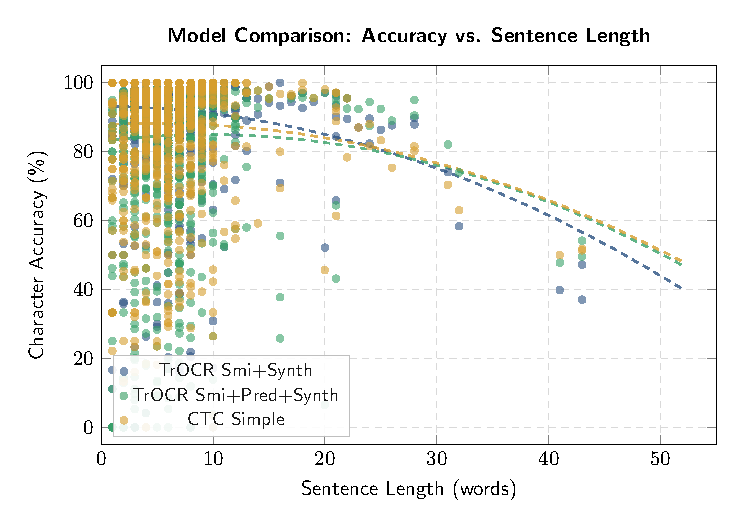
\includegraphics[width=\columnwidth]{figures/model_comparison_sentence_length.pdf}
    \caption{\footnotesize Character accuracy vs. sentence length for TrOCRs (trocr\_smi\_synth, trocr\_smi\_pred\_synth) and  ctc\_simple models. Both architectures degrade beyond $\sim$\sentenceLengthThreshold{} characters due to fixed \preprocessingImgWidth{} pixel input width compressing longer text. Points are single test samples, lines are regression trends.}
    \label{fig:length_analysis}
\end{figure}
% \begin{figure}[t]
%     \centering
%     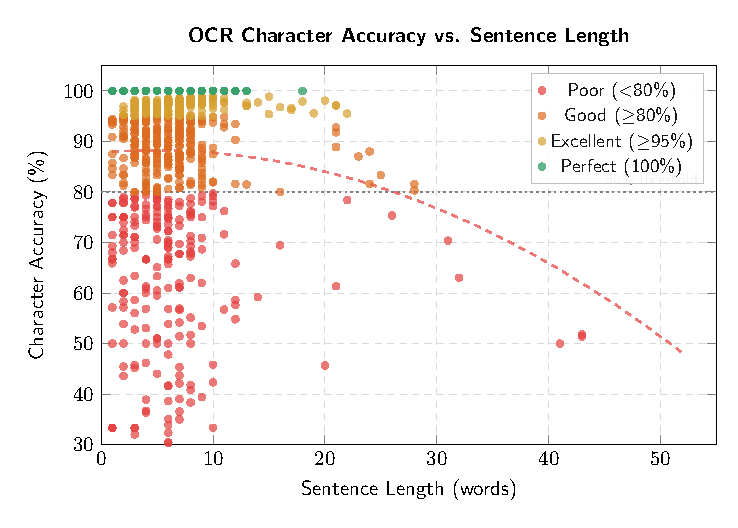
\includegraphics[width=\columnwidth]{figures/sentence_length_analysis.pdf}
%     \caption{Character accuracy versus sentence length for TrOCR (trocr\_smi\_synth) and CNN-CTC (ctc\_simple) models. Both architectures degrade beyond $\sim$\sentenceLengthThreshold{} characters due to fixed \preprocessingImgWidth{} pixel input width compressing longer text. Points show individual test samples, lines show local regression trends.}
%     \label{fig:length_analysis}
% \end{figure}

Both architectures exhibit degrading accuracy with increasing sentence length, with a critical threshold around \sentenceLengthThreshold{} to 100 characters. This degradation stems from the fixed \preprocessingImgWidth{} pixel input width: longer sentences are compressed into the same pixel budget, reducing effective resolution per character.

For sentences under \sentenceLengthThreshold{} characters, TrOCR(trocr\_smi\_synth) maintains higher accuracy but with greater variance. The CTC model shows more consistent performance across all lengths, likely due to its simpler architecture being less sensitive to input compression artifacts.

\textbf{Conjunction-Based Splitting Mitigation:} To address this length-based degradation, we implement a linguistically motivated preprocessing approach: splitting long sentences at North S\'{a}mi conjunction boundaries before OCR, then rejoining predictions. North S\'{a}mi uses coordinate conjunctions (\textit{ja} ``and'', \textit{muhto} ``but'', \textit{dahje} ``or'') and subordinate conjunctions (\textit{go} ``when/because'', \textit{ahte} ``that'', \textit{jos} ``if'')~\cite{valijarvi2013} that naturally delimit clause boundaries. Only texts exceeding \sentenceLengthThreshold{} characters are processed, splitting \textit{before} conjunctions, maintaining minimum segment lengths of 20 characters to avoid over-splitting. 

% Table~\ref{tab:split_experiment} shows the results.
Figure~\ref{fig:split_comparison} shows the results. 
For long sentences ($>$\sentenceLengthThreshold{} characters, $n$=\splitLongCount{}), conjunction-based splitting dramatically reduces CER from \splitLongOriginalCER\% to \splitLongSplitCER\%, an improvement of \splitImprovement{} percentage points. What is noteworthy, is that this brings long sentence CER \textit{below} that of short sentences (8.12\% vs 12.04\%), effectively eliminating the length penalty. A paired t-test confirms statistical significance ($p = \splitPValue{}$) with a large effect size (Cohen's $d = \splitCohensD{}$). Critically, \splitImproveRate\% of split samples showed improvement with no degradation cases. Because the splitter operates on ground truth, this is an oracle upper bound: a deployed system would have to detect conjunctions on noisy OCR output, so only a fraction of the gain would carry over. We therefore present conjunction splitting as a proof of concept.

% \begin{table}[t]
% \centering
% \caption{Conjunction-Based Splitting Results (ctc\_simple)}
% \label{tab:split_experiment}
% \small
% \begin{tabular}{@{}lccc@{}}
% \toprule
% \textbf{Sentence Type} & \textbf{Original CER} & \textbf{Split CER} & \textbf{$\Delta$} \\
% \midrule
% Long ($>$80 chars) & \splitLongOriginalCER\% & \splitLongSplitCER\% & \textbf{-\splitImprovement pp} \\
% \bottomrule
% \end{tabular}

% \vspace{0.3em}
% \footnotesize{$n$=\splitLongCount{} long sentences, \splitSamplesSplit{} split. Paired $t$-test: $p$=\splitPValue{}, $d$=\splitCohensD{}.}
% \end{table}

\begin{figure}
    \centering
    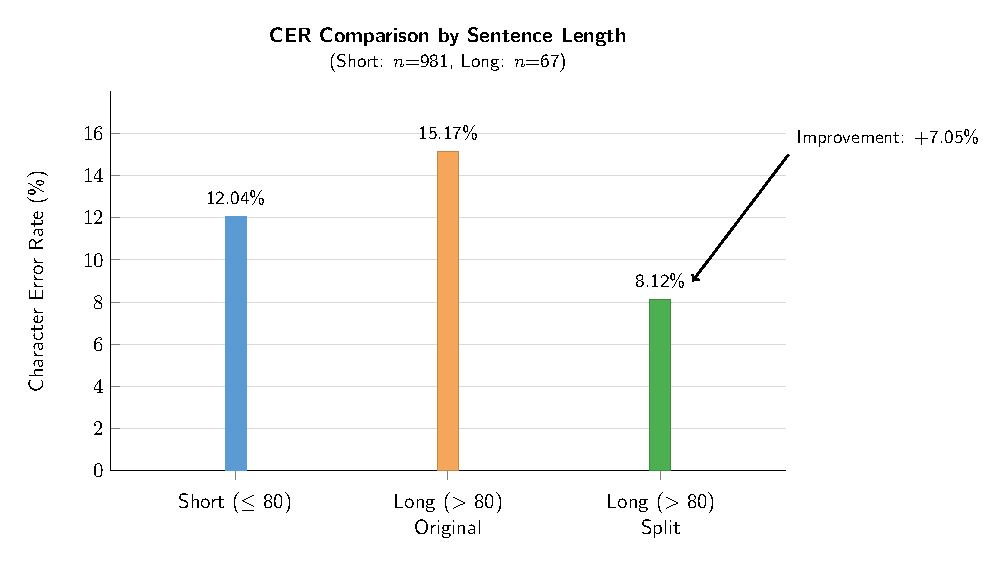
\includegraphics[width=\columnwidth]{figures/split_comparison.pdf}
    \caption{\footnotesize CER comparison showing the effect of conjunction-based splitting. Long sentences ($>$\sentenceLengthThreshold{} chars) degrade to \splitLongOriginalCER\% CER when processed whole, but splitting at conjunction boundaries reduces error to \splitLongSplitCER\%, even better than short sentences (\splitShortCER\%).}
    \label{fig:split_comparison}
\end{figure}



Table~\ref{tab:split_example} illustrates this improvement with a concrete example from Turi's work. A 137-character sentence, when processed whole, truncates after $\sim$110 characters (19.7\% CER). The splitter detects a subordinate conjunction \textit{go} (``when/because'') and divides the input in 2 segments, each processed independently, then rejoined to achieve 0\% CER.

\begin{table}[tb]
\centering
\caption{\footnotesize Split Example: Conjunction-Based Segmentation}
\label{tab:split_example}
\small
\begin{tabular}{@{}p{0.95\columnwidth}@{}}
\toprule
\textbf{Ground Truth} (137 chars) \\
\textit{Ja dasa lea d\'{a}t sivva: \textbf{go} s\'{a}pmela\v{s} boaht\'{a} moskkus g\'{a}mmirii, de son ii ipmir ii b\'{a}ljo maidege, \textbf{go} ii biegga beasa bossut njuni vuost\'{a}.} \\
\midrule
\textbf{Original Prediction} (19.7\% CER) \\
\textit{Ja dasa lea d\'{a}t sivva: go s\'{a}pmela\v{s} boaht\'{a} moskkus g\'{a}mmirii, de son ii ipmir ii b\'{a}ljo maidege, go ii biegga bea}\\
\midrule
\textbf{Split Processing} $\rightarrow$ \textbf{Rejoined} (0.0\% CER) \\
% \footnotesize
\textbf{Seg.\ 1:} \textit{Ja dasa lea d\'{a}t sivva: go s\'{a}pmela\v{s} boaht\'{a} moskkus g\'{a}mmirii, de son ii ipmir ii b\'{a}ljo maidege,} \\
\textbf{Seg.\ 2:} \textit{go ii biegga beasa bossut njuni vuost\'{a}.} \\
% \normalsize
\textbf{Joined}\textit{$\hookrightarrow$ Ja dasa lea d\'{a}t sivva: go s\'{a}pmela\v{s} boaht\'{a} moskkus g\'{a}mmirii, de son ii ipmir ii b\'{a}ljo maidege, go ii biegga beasa bossut njuni vuost\'{a}.} \\
\bottomrule
\end{tabular}
\vspace{0.2em}
\footnotesize{Split at second \textit{go} conjunction, each segment fits within 800px width constraint.}
\end{table}

This finding suggests that simple, linguistically informed preprocessing can substantially mitigate the length constraint without architectural changes. We hypothesize this approach generalizes to other agglutinative languages with similar clause-marking conjunctions.

\subsection{End-to-End Pipeline Evaluation}
\label{subsec:pipeline}

To demonstrate practical applicability, we evaluated a proof-of-concept OCR$\rightarrow$MT pipeline using the TartuNLP neural machine translation API~\cite{tartunlp} to translate predicted North S\'{a}mi text to English. Using \textit{ctc\_simple} OCR outputs, the pipeline achieved BLEU~\cite{post2018call} \bleuScore{}, chrF~\cite{popovic2015chrf} \chrfScore{}, and TER \terScore{}\%.

These moderate translation scores reflect the cascading effect of OCR errors: a \ctcCER\% character error rate propagates through to mistranslations and reduced fluency.
Qualitative analysis shows that OCR errors in morphological suffixes (e.g., case markers) disproportionately affect MT output, as the agglutinative structure means single character errors can change grammatical relations.
Additionally, this highlights the need for reliable, open-access translation tools bridging high-resource languages such as English and low-resource languages like S\'{a}mi. Nevertheless, the system can process historical documents end-to-end without manual transcription, providing rough translations suitable for archival indexing.


\subsection{Error Analysis}
\label{sec:error_analysis}

Qualitative examination of prediction errors reveals several patterns, illustrated in Table~\ref{tab:ocr_examples}.

\begin{table}[t]
\centering
\caption{\footnotesize OCR Recognition Examples with Ground Truth Images (ctc\_simple model)}
\label{tab:ocr_examples}
\small
\begin{tabular}{@{}p{\columnwidth}@{}}
\toprule
\textbf{Correct Recognition (CER = 0\%)} \\
\midrule
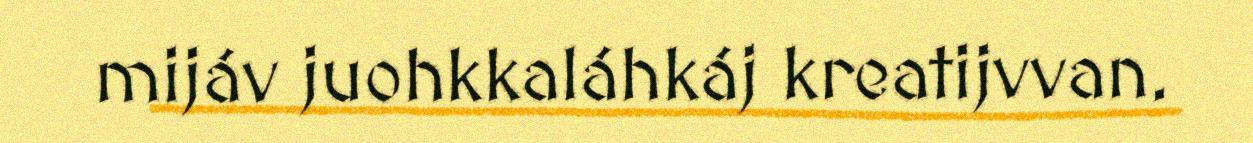
\includegraphics[width=\columnwidth]{./figures/ground_truth/correct2.jpg} \\
\textbf{Ground Truth:}  \textit{mij\'{a}v juohkkal\'{a}hk\'{a}j kreatijvvan.} \\
\textbf{Prediction:} \textit{mij\'{a}v juohkkal\'{a}hk\'{a}j kreatijvvan.} \\
% \midrule

\includegraphics[width=\columnwidth]{./figures/ground_truth/correct1.jpg} \\
\textbf{Ground Truth:}  \textit{julev- ja davvis\'{a}migielagiiguin ja s\'{a}miiguin geat eai} \\
\textbf{Prediction:} \textit{julev- ja davvis\'{a}migielagiiguin ja s\'{a}miiguin geat eai} \\
\midrule
\textbf{Diacritical Errors (CER = 8.3\%)} \\
\midrule

\includegraphics[width=\columnwidth]{./figures/ground_truth/diacritical_errors_new.jpg} \\
\textbf{Ground Truth:} \textit{ođđasis eal\'{a}skahttojuvvon) Suohkana h\'{a}lddahusla\v{s}} \\ %\dj\dj 
\textbf{Prediction:} \textit{oddasis eal\'{a}skahttojuvvon) Duohkama h\'{a}lddahusla\v{s}} \\
\footnotesize{Note: ođđasis $\rightarrow$ oddasis shows đ$\rightarrow$d error (stroke missed)} \\ %\dj\dj
% \normalsize
% \textbf{Diacritical Errors (CER = 14.5\%)} \\
% \midrule
% 
\includegraphics[width=\columnwidth]{./figures/ground_truth/diacritical_errors.jpg} \\
% \textbf{Ground Truth:} \textit{mearr\'{a}dusa. S\'{a}medikker\'{a}\dj\dj i lea v\'{a}iddaorg\'{a}na \'{a}\v{s}\v{s}iide mat} \\
% \textbf{Prediction:} \textit{marr\'{a}dusa. D\'{a}mediblor\'{a}\dj\dj i lea v\'{a}iddaorg\'{a}ma \'{a}\v{s}\v{s}ie mat} \\
\midrule
\textbf{Uppercase Text Errors (CER = 29.6\%)} \\
\midrule

\includegraphics[width=\columnwidth]{./figures/ground_truth/uppercase_errors.jpg} \\
\textbf{Ground Truth:} \textit{FYLKKAGIELDDAIGUIN. FINNM\'{A}RKKU FYLKKAGIELDDAS LEA \'{A}IGUMU\v{S}\v{S}IEHTADUS S\'{A}MI} \\
\textbf{Prediction:} \textit{FYLKKAGIELDDAIGUI0. F1O0m\'{A}RKKU FYLKKAGIELDDAs LEA \'{A}IGUmU\v{S}e} \\
\bottomrule
\end{tabular}
\end{table}


\textbf{ImageNet-Pretrained Models:} The three CTC models using ImageNet-pretrained backbones (ctc\_vgg16: 73.9\% CER, ctc\_vgg19: 71.9\% CER, ctc\_resnet50: 75.3\% CER) did not converge to usable performance despite using the same projection layer and CTC head as ctc\_simple. All three models achieved 0\% exact match accuracy, producing largely unintelligible character sequences.

% We hypothesize that the failure is stemming from the pre-training, where the model was prepared to recognise existing objects and shapes and not length-varying text. % my personal hypothesis
We hypothesize that ImageNet's object-level features (edges, textures, boundaries) misalign with character-level recognition (stroke topology, diacritics, spacing), while SimpleCNN trained from scratch learns task-appropriate features. The 70 to 75\% vs 12.24\% CER gap points to a representation problem rather than under optimization, though this conclusion holds only under our compute budget.


\textbf{Consonant Clusters:} The CTC model occasionally drops characters in complex consonant clusters common in S\'{a}mi morphology (e.g., predicting ``sggoda'' for ``cuiggoda''). TrOCR handles these better, likely due to its decoder's language modeling capacity. Post-correction integration could mitigate this issue (See Section ~\ref{sec:conclusion}). 

\textbf{Diacritical Character Handling:} Table~\ref{tab:diacritics} presents per-character accuracy for the seven S\'{a}mi-specific diacritics. TrOCR(trocr\_smi\_synth) achieves 93.4\% overall diacritic accuracy compared to the CTC model's 88.3\%. Both models struggle most with ŧ (50\% accuracy), likely due to its visual similarity to standard `t' and extreme rarity in the test set (only 6 occurrences). Interestingly, the CTC model achieves perfect accuracy on ŋ (26 occurrences) while TrOCR confuses it with `g' (84.6\%). The high accuracy on \'{a} (90 to 96\%) benefits from its frequency (1,473 occurrences). Common error patterns include \'{a}$\rightarrow$a diacritic stripping, đ$\rightarrow$d confusion (the stroke being missed), and case confusions (e.g., \'{A}$\leftrightarrow$\'{a}).


\textbf{Case Sensitivity:} Both models struggle with all uppercase text (a small part of training samples). This suggests a need for case-augmented training or case normalization preprocessing. 

\textbf{Length-Dependent Errors:} As shown in Figure~\ref{fig:length_analysis}, both models degrade on sentences exceeding \sentenceLengthThreshold{} characters due to the fixed \preprocessingImgWidth{} pixel input width constraint discussed in Section~\ref{subsec:preprocessing} with mitigation technique in Section~\ref{subsec:length_analysis}.


\begin{table}[h]
    \centering
    \caption{\footnotesize Per-Character Accuracy for S\'{a}mi Diacritics}
    \label{tab:diacritics}
    \small
    \begin{tabular}{@{}lccc@{}}
    \toprule
    \textbf{Character} & \textbf{Count} & \textbf{ctc\_simple} & \textbf{trocr\_smi\_synth} \\
    \midrule
    \'{a} / \'{A} & 1473 & 90.1\% & 95.9\% \\
    \v{c} / \v{C} & 129 & 83.7\% & 81.4\% \\
    đ / Đ & 191 & 79.1\% & 87.4\% \\
    ŋ / Ŋ & 26 & 100.0\% & 84.6\% \\
    \v{s} / \v{S} & 262 & 87.8\% & 93.1\% \\
    ŧ / Ŧ & 6 & 50.0\% & 50.0\% \\
    \v{z} / \v{Z} & 35 & 80.0\% & 85.7\% \\
    \midrule
    \textbf{Overall} & 2122 & 88.3\% & 93.4\% \\
    \bottomrule
    \end{tabular}
\end{table}

% ============================================================================
% VI. DISCUSSION (~0.8 pages)
% ============================================================================

\section{Discussion}
\label{sec:discussion}

\subsection{Practical Deployment Considerations}
\label{subsec:deployment}

Our lightweight CNN-CTC model paves the way for deployment scenarios where TrOCR remains impractical. At \ctcThroughputK{},000 images per hour, a single CPU can process a million pages in under \millionPagesCtcHours{} hours vs. \millionPagesTrocrDays{} days for TrOCR, allowing cultural institutions to complete S\'{a}mi digitization projects with reasonable time and budget. The \ctcSize{}MB footprint permits deployment on mobile devices for field documentation in remote areas, supporting indigenous data sovereignty by avoiding cloud-based processing. Latency below 100ms enables interactive transcription interfaces with immediate feedback.

While TrOCR may be preferable for cases where precision is paramount, the \cerGap{}pp CER gap represents an acceptable trade off for bulk indexing and content discovery. Our model's stable performance on synthetically rendered historical lexical content (Section~\ref{subsec:generalization}) suggests practical reliability may exceed what synthetic benchmarks alone indicate.

\subsection{Limitations}
\label{subsec:limitations}

There are several limitations constraining the present work. All models were trained on synthetic data rather than real scans, while historical evaluation (Section~\ref{subsec:generalization}) demonstrates lexical generalization, performance on physical degradation (faded ink, paper damage) remains untested and requires a corpus of real scanned S\'{a}mi documents. The pre-segmentation of text lines is assumed, which requires layout analysis tool integration for full-page processing, and the fixed \preprocessingImgWidth{} pixel OCR width constrains very long lines. Additionally, our models perform pure vision-based OCR without morphological post-correction. Integrating Giellatekno's analyzer~\cite{moshagen2014} could improve accuracy for rare inflected forms.

We did not evaluate classical OCR baselines (Tesseract, Transkribus), our focus was on comparing lightweight neural architectures against state-of-the-art Transformer models. Enstad et al.~\cite{enstad2025} provides Tesseract comparisons showing substantially higher CER ($>$30\%) on S\'{a}mi text.

\subsection{Ethical Considerations}
\label{subsec:ethics}

This work addresses language technology for a historically marginalized community. Following the years of policies that suppressed S\'{a}mi languages, revitalization is a matter of cultural survival and historical justice. Technology must support, not replace, community efforts. Our edge-deployable model enables local processing without uploading sensitive materials to external servers. We provide our work results to benefit institutions and communities, highlighting the need to prevent commercial exploitation of indigenous language resources.
Following the CARE Principles for Indigenous Data Governance~\cite{carroll2020care}, emphasizing Collective Benefit, Authority to Control, Responsibility, and Ethics, we commit to releasing models and code under the MIT license via GitHub and HuggingFace. 
All source material consists of published historical texts in the public domain. Formal Free, Prior and Informed Consent (FPIC) was not required as no unpublished community materials were used. 

% ============================================================================
% VII. CONCLUSION AND FUTURE WORK (~0.5 pages)
% ============================================================================
\section{Conclusion and Future Work}
\label{sec:conclusion}

This work demonstrates that lightweight CNN-CTC architectures offer viable, high-efficiency alternatives to Transformer-based architectures for North S\'{a}mi OCR. Our \texttt{ctc\_simple} model achieves \ctcCER\% CER, only \cerGap{}pp behind the best TrOCR variant, while operating \speedupFactor$\times$ faster with a \sizeRatio$\times$ smaller footprint, enabling high-throughput (\ctcThroughputK{},000 images/hour on CPU), making large-scale digitization feasible. 
%While our evaluation lays within the historical lexical content, we showcase that the architecture's possible applications are diverse. 
Notably, our lightweight model exhibits stable performance on \turiYear{} historical text ($n=$\bookTestSamples{}) while TrOCR degrades by \trocrSynthDeltaCER{}pp, suggesting that smaller architectures may generalize better to domain-specific features than Transformers. We find that pretrained generic ImageNet backbones fail to converge in this task, indicating that training a model from scratch may better suit specialized indigenous language recognition. Linguistically motivated sentence splitting mitigates length-based degradation under oracle conditions ($p < 0.00001$), indicating a promising preprocessing direction that remains to be validated on predicted text. 
%End to end OCR$\rightarrow$MT evaluation confirms OCR accuracy as the primary translation bottleneck.

% \begin{figure}[t]
%     \centering
%     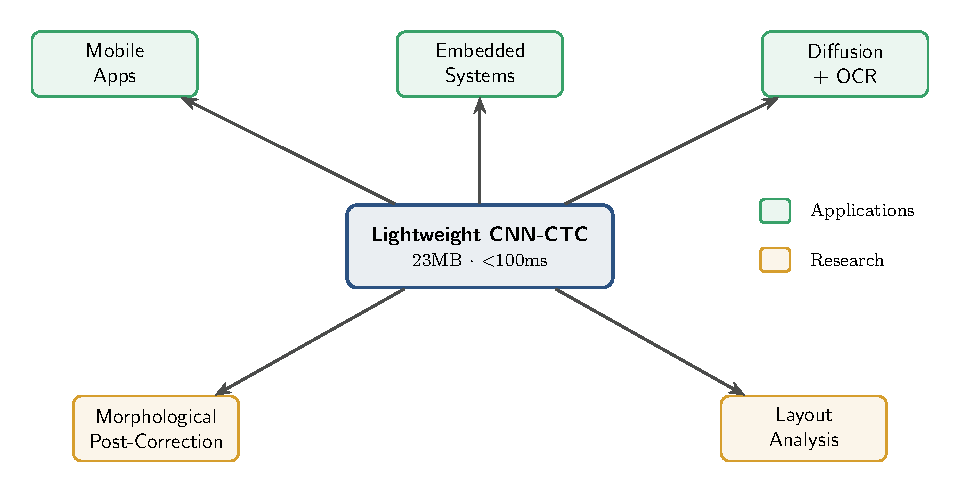
\includegraphics[width=\columnwidth]{figures/future_work.pdf}
%     \caption{Targeted applications: From the lightweight CNN-CTC model to practical applications (mobile tools, embedded systems) to research extensions (morphological post-correction, layout analysis)}
%     \label{fig:future_work}
% \end{figure}
\begin{figure}[tb]
    \centering
    \begin{subfigure}[b]{\columnwidth}
        \centering
        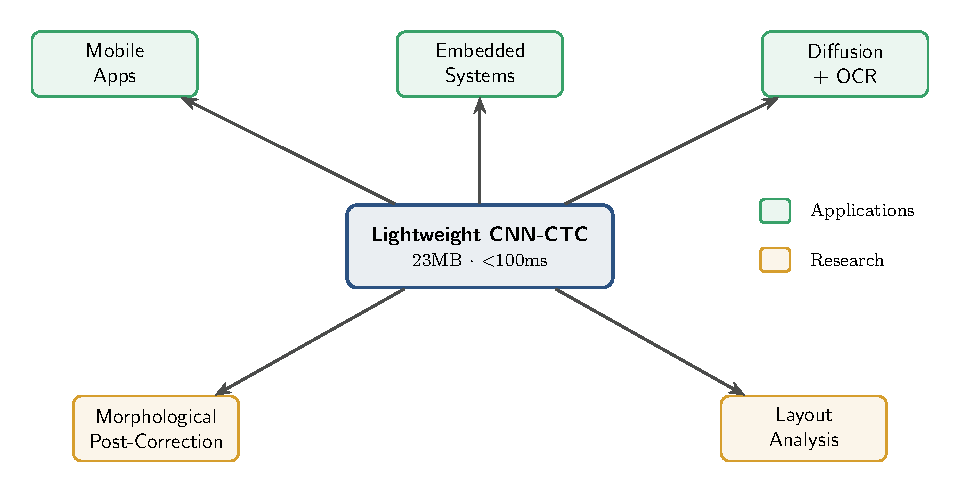
\includegraphics[width=\columnwidth]{figures/future_work.pdf}
        % \caption{From the lightweight CNN-CTC model to practical applications (mobile tools, embedded systems) and research extensions (morphological post-correction, layout analysis).}
        \label{fig:future_work}
    \end{subfigure}
    \begin{subfigure}[b]{\columnwidth}
        \centering
        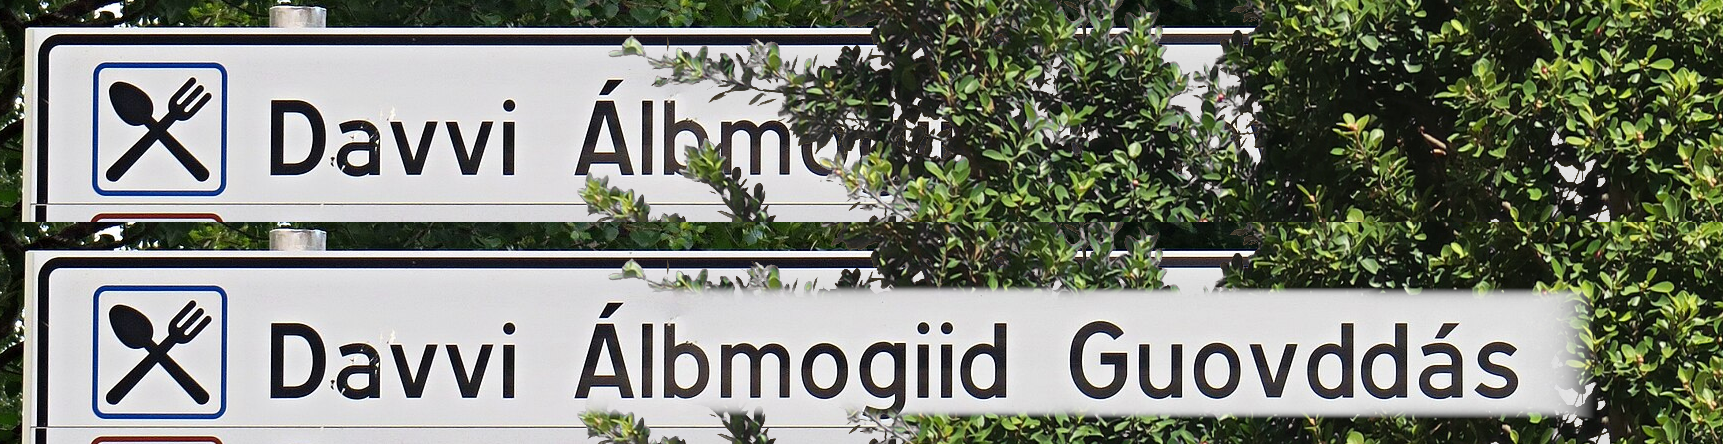
\includegraphics[width=\columnwidth]{figures/reconstruction.png}
        % \caption{Reconstruction example: occluded road sign and expected reconstruction.}
        \label{fig:reconstruction}
    \end{subfigure}

    \caption{\footnotesize (a) Targeted applications and future directions for our lightweight OCR model, (b) Potential use case in damaged text reconstruction, e.g. in autonomous driving (this can also be useful for grocery store labels etc.)}
    \label{fig:applications}
\end{figure}
% \vspace{-1.2em}

Figure~\ref{fig:applications} summarizes targeted applications of this work. In the future, combining a diffusion model and existing OCR solution can yield unified pipelines for damaged text reconstruction. Through small size ($\ctcSize{}$MB) and low latency ($< 100$ms), this is deployable on embedded devices useful in self-driving vehicles when road signs are occluded or organizing of shop items with damaged labels.       
Our model's portability makes it suitable for mobile applications in document digitization, useful in areas without internet connectivity. To improve accuracy, especially for rare inflected forms, a Giellatekno's morphological analyzer~\cite{moshagen2014} for post-correction can be integrated, though it needs corpora of real scanned documents to train authentic degradation artifacts. Line-level OCR can be combined with layout analysis (de-skewing, line detection) to enable full-page document processing. 
Future work can also entail implementation of some targeted applications, especially to train next-gen robots. Further related exploration can be in languages with challenges of fully pictorial scripts~\cite{dong2021} and in aspects such as cultural commonsense~\cite{nguyen2023} as well as human-robot collaboration using text \& images~\cite{DISCERN2024}, possibly collating with earlier work by our research teams. 

Our research in this paper is noteworthy for impacts on 21st-century education by addressing resource-aware OCR in indigenous low-resource languages. It aids smart learning \& smart living due to the usefulness of the OCR transcription and its targeted applications. 

% \begin{figure}[t]
%     \centering
%     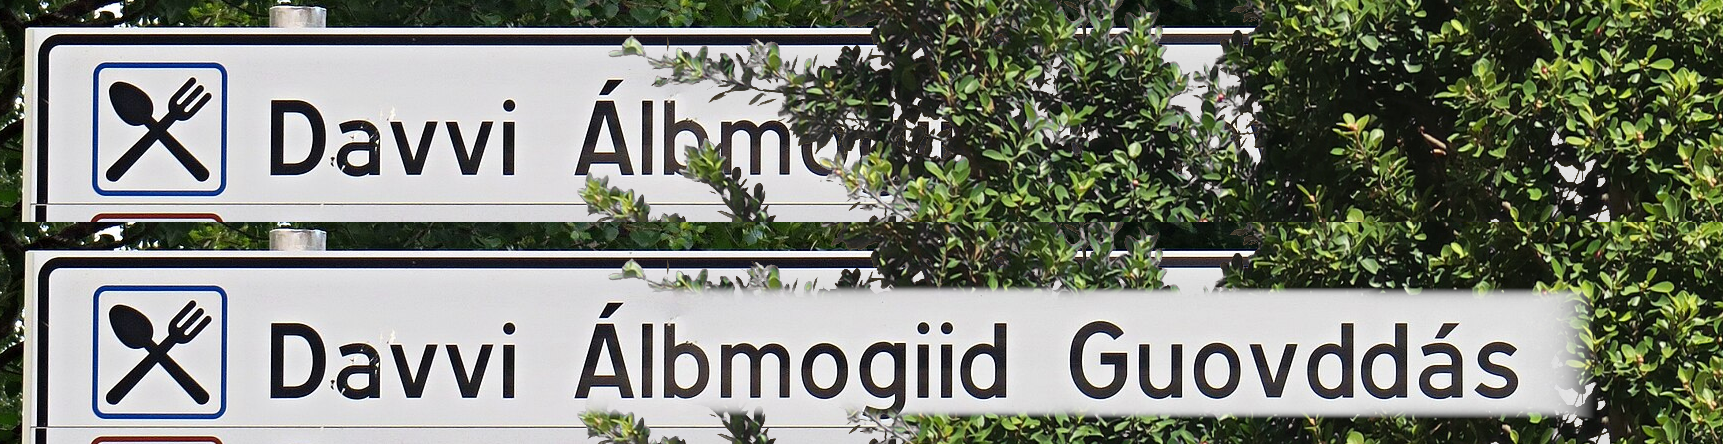
\includegraphics[width=\columnwidth]{figures/reconstruction.png}
%     \caption{Reconstruction Example: the occluded road sign and expected reconstruction of it.}
%     \label{fig:reconstruction}
% \end{figure}


\section*{Acknowledgments}
\footnotesize

We thank the National Library of Norway (Spr\r{a}kbanken) for providing pre-trained TrOCR models and synthetic training data. We acknowledge Giellatekno (UiT The Arctic University of Norway) for the SIKOR corpus and test data. We thank TartuNLP (University of Tartu) for providing the North S\'{a}mi to English translation API. Computational resources were provided by the University of Southern Denmark. Aparna Varde acknowledges a grant from NNF, Denmark, in the area of Sustainable AI. 


% ============================================================================
% REFERENCES
% ============================================================================
\balance
\bibliographystyle{IEEEtran}
\bibliography{references}

\end{document}